\section{Análise Quantitativa do algoritmo - SCP}

\noindent
Para que pudesse ser feita uma análise quantitativa completa, seria necessário ter uma
proposta de código finalizada, o que não é o caso. Para que possa se ter essa proposta,
é preciso fazer uma avaliação fina tanto do funcionamento do método como um todo, quanto
com cada parte isolada, com um foco especial na busca da direção de descida e no ajuste
das constantes de penalidade presentes em todo o processo. No entanto, será apresentado
resultados que consideramos parciais acerca do custo de processamento.
% , fazendo um comparativo simples com um método simples, o gradiente descendente. Para que se possa ser usado o método do gradiente descendente em problemas com restrições será usado a função Lagrangiana do problema
O código de nossa autoria que foi construído como uma proposta para o SCP é
o que usamos nos testes, e este está disponível publicamente em um repositório no Github
\footnote{Disponível em: \url{https://github.com/Sekva/tcc_prog/tree/56fa674}}.

Para os testes, foram usados 10 problemas de 3 bases de dados diferentes.
Duas dessas bases de dados foram as mesmas usadas pelos desenvolvedores do
SCP, uma compilada por Hock e Schittkowski \cite{Hock1981}
e Schittkowski \cite{Schittkowski1987}. Enquanto a elaboração do teste, apenas são
considerados problemas cujo domínio é o \(\mathbb{R}^2\), e problemas com ambas as
restrições, tanto de igualdade quanto de desigualdade, por simplicidade e
verificação da consistência entre problemas. Dado o estado atual da implementação do
método, não foi vista a necessidade de apresentação do ponto supostamente ótimo
encontrado pelo algoritmo para cada um dos problemas apresentados. No entanto,
será falado a respeito das implicações acerca do que foi encontrado.

Todos os testes foram feitos em uma CPU AMD FX-6300, no sistema operacional
ArchLinux-2021.06.01. O compilador usado foi o rustc 1.51.0-nightly, edição 2018,
compilação não otimizada e informações de debug. A não otimização e a preservação
das informações de debug do programa são feitas para que se possa usar um debugger
mais facilmente e evitar o rearranjo de código por parte do compilador, uma vez
que durante a compilação as otimizações feitas podem alterar drasticamente a
ordem das operações executadas a fim de garantir a maior eficiência possível
para as operações de baixo nível.

\subsection{Problemas de Surjanovic e Bingham}

\noindent
A primeira base de problemas considerada \cite{sfuca} é parte de um projeto colaborativo
para se ter uma biblioteca de funções e conjuntos de dados para testes em diversas
áreas de otimização, simulação e modelagens em geral. Foram escolhidos quatro
problemas da base por serem problemas simples, os quais estão listados na Tabela \ref{sfuca_probs}. No entanto, são todos irrestritos,
isto é, consistem apenas em minimizar a função sem nenhuma restrição.

{
  \bgroup
  \def\arraystretch{2}%  1 is the default, change whatever you need
  \begin{table}[H]
    \centering
    \vspace{6pt}
    \caption{Funções de teste irrestritas.\label{qua:funcoes-irrestritas}}
    \vspace{6pt}
    \begin{tabular}{||c|c|c||} 
      \hline
      Nome        & Expressão & Ótimo (\(x^*\)) \\ [0.5ex] 
      \hline\hline
      Bohachevsky & \(\displaystyle{f(x) = x_1^2 + 2x_2^2 - 0.3 \cos(3 \pi x_1 + 4 \pi x_2) + 0.3} \)                    & \((0, 0)\) \\ 
      \hline
      Perm        & \(\displaystyle{f(x) = \sum_{i=1}^2 \left( \sum_{j=1}^2 (j+\beta) x_j^i - \frac{1}{j^i}\right)^2} \) &  \((1, \frac{1}{2})\) \\
      \hline
      Trid        & \(\displaystyle{f(x) = \sum_{i=1}^2 (x_i - 1)^2 - \sum_{i=2}^2 x_i x_{i-1}} \)                       & \((2, 2)\) \\
      \hline
      Sum Squares & \(\displaystyle{f(x) = \sum_{i=1}^2 ix_i^2} \)                                                       & \((0, 0)\) \\ [1ex]
      \hline
    \end{tabular}
    \label{sfuca_probs}
  \end{table}
}

\begin{center}

  \vspace{6pt}
  \captionof{figure}{Função de Bohachevsky com ótimo em (0, 0).}
  \label{boha_fig}
  \vspace{6pt}
  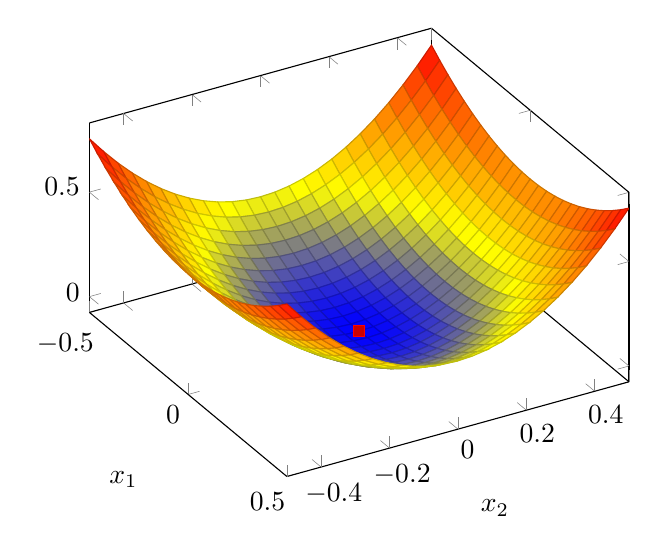
\begin{tikzpicture}
    \begin{axis}[xlabel=$x_1$,ylabel=$x_2$,domain=-0.5:0.5, y domain=-0.5:0.5,view/h=60,view/v=45,]
      % \addplot3 [surf,mesh/ordering=y varies,] {x^2 + 2*y^2 - 0.3 * cos(3 * 3.14159626 * x + 4 * 3.1415926 *  y) + 0.3};
      \addplot3 [surf,mesh/ordering=y varies,] { x^2 - (0.3 * cos(((9.42479 * x) + (12.5664 * y)))) + (2 *  y^2) + 0.3 };
      \addplot3+ [only marks] coordinates {(0, 0, 0)};
    \end{axis}
  \end{tikzpicture}

  \vspace{6pt}
  \captionof{figure}{Função Perm com ótimo em (1, 0.5).}
  \label{perm_fig}
  \vspace{6pt}
  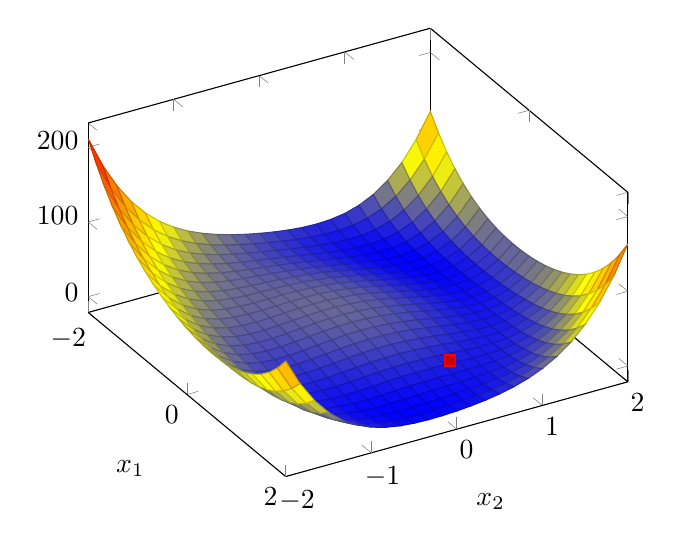
\begin{tikzpicture}
    \begin{axis}[xlabel=$x_1$,ylabel=$x_2$,domain=-2:2, y domain=-2:2,view/h=60,view/v=45,]
      \addplot3 [surf,mesh/ordering=y varies,] {(((1+0.5)*x-1)+((2+0.5)*y - 0.5) )^2 + (((1+0.5)*x^2-1)+((2+0.5)*y^2-4))^2 };
      \addplot3+ [only marks] coordinates {(1, 0.5, 0)};
    \end{axis}
  \end{tikzpicture}

  \vspace{6pt}
  \captionof{figure}{Função Trid com ótimo em (2, 2).}
  \label{trid_fig}
  \vspace{6pt}
  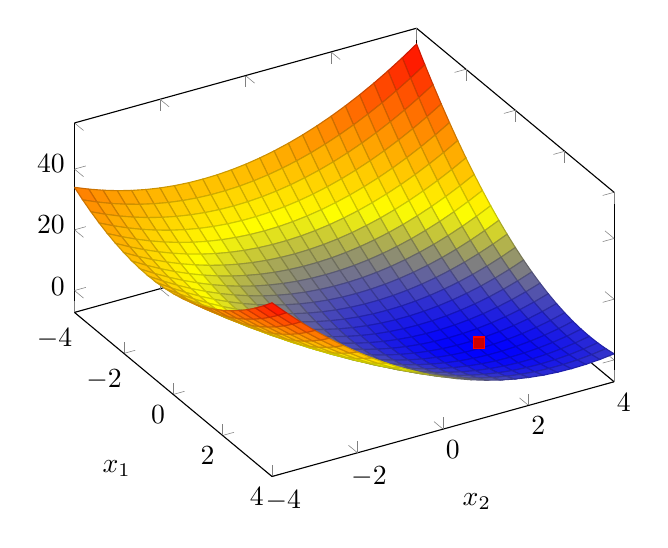
\begin{tikzpicture}
    \begin{axis}[xlabel=$x_1$,ylabel=$x_2$,domain=-4:4, y domain=-4:4,view/h=60,view/v=45,]
      \addplot3 [surf,mesh/ordering=y varies,] {(x-1)^2 + (y-1)^2  - y*x};
      \addplot3+ [only marks] coordinates {(2, 2, 0)};
    \end{axis}
  \end{tikzpicture}

  \vspace{6pt}
  \captionof{figure}{Função Sum Squares com ótimo em (0, 0).}
  \label{sumsquares_fig}    
  \vspace{6pt}
  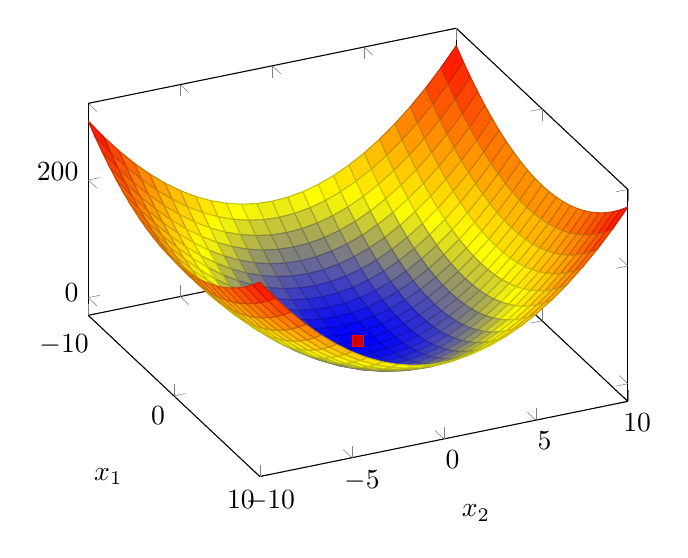
\begin{tikzpicture}
    \begin{axis}[xlabel=$x_1$,ylabel=$x_2$,domain=-10:10, y domain=-10:10,view/h=65,view/v=40,]
      \addplot3 [surf,mesh/ordering=y varies,] {  (1 * x^2) + (2 * y^2)   };
      \addplot3+ [only marks] coordinates {(0, 0, 0)};
    \end{axis}
  \end{tikzpicture}
  
\end{center}

Como todos os problemas são irrestritos, foram consideradas restrições simples.
Para as restrições de desigualdade, foram consideradas quatro funções limitando o
ponto a um quadrado em uma distância razoável do ótimo. Para as restrições de
igualdade, basta considerar uma função que passe no ótimo, a mais simples é
apenas uma reta. Devemos lembrar que estamos trabalhando apenas no \(\mathbb{R}^2\).

Cada uma das funções buscam testar o funcionamento da descida do método em superfícies
com características diferentes. A função de Bohachevsky (Figura \ref{boha_fig}) tem uma
superfície com lombadas, causadas pela função trigonométrica em sua definição, o que faz
verificar se o processo não fica preso em um ótimo local. A função de Perm (Figura \ref{perm_fig})
tem uma especie de anel em que o mínimo está localizando, verificando se o método é capaz
de contornar ou atravessar esse anel. A função Trid (Figura \ref{trid_fig}) tem uma
inclinação diferente em cada direção, o que serve de apoio para a análise das direções de
descidas encontradas durante os testes. Por fim, a função Sum Squares
(Figura \ref{sumsquares_fig}) é apenas um paraboloide elíptico de rápida descida.



\subsection{Problemas de  Hock e Schittkowski}

\noindent
As outras duas bases de testes são compilações de funções usadas ao longo de anos
de estudos sobre métodos de resolução de problemas não lineares dos autores. Segundo
eles, o livro onde é apresentada a base de dados deve ser considerado uma assistência
para o design de testes, uma vez que a performance só pode ser medida de fato através
de experiência numérica, a qual se faz necessário ter uma coleção de problemas para
que exista uma experiência.

Da primeira base, foram escolhidos os seguintes problemas:


\begin{subequations}
  \label{prob_h1}
  \begin{align}
    \hspace*{0pt}\hfill \underset{x}{\text{min}} \hspace{0.2cm} & f(x) = 100(x_2 - x_1^2)^2 + (1-x_1)^2 \hspace{2.85cm} \\
    \hspace*{0pt}\hfill \text{s.a} \hspace{0.2cm} & 1.5 \leq x_2 \hspace{2.85cm} \\
    \hspace*{0pt}\hfill & \hspace{0.15cm} x^* = (1, 1) \hspace{2.85cm} 
  \end{align}
\end{subequations}

% \begin{mini!}
%   {x}{f(x) = 100(x_2 - x_1^2)^2 + (1-x_1)^2}{\label{prob_h1}}{}
%   \addConstraint{1.5}{\leq x_2}{}
%   \addConstraint{x^*}{= (1, 1)}{}
% \end{mini!}

\vspace{-0.5cm}

\begin{subequations}
  \label{prob_h2}
  \begin{align}
    \hspace{0pt}\hfill \underset{x}{\text{min}} \hspace{0.2cm} & f(x) =   (x_1 - 2)^2 + (x_2-1)^2 \\
    \hspace{0pt}\hfill \text{s.a} \hspace{0.2cm} & -0.25x_1^2 - x_2^2 + 1 \geq 0 \\
    \hspace{0pt}\hfill & \hspace{1cm} x_1 - 2x_2 + 1 = 0 \\
    \hspace{0pt}\hfill & \hspace{2.85cm} x^* = (0.5(\sqrt{7}-1), 0.25(\sqrt{7}+1))
  \end{align}
\end{subequations}




% \begin{mini!}
%   {x}{f(x) =  (x_1 - 2)^2 + (x_2-1)^2 }{\label{prob_h2}}{}
%   \addConstraint{-0.25x_1^2 - x_2^2 + 1}{\geq 0}{}
%   \addConstraint{x_1 - 2x_2 + 1}{= 0}{}
%   \addConstraint{x^*}{= (0.5(\sqrt{7}-1), 0.25(\sqrt{7}+1))}{}
% \end{mini!}




O problema (\ref{prob_h1}) é o Problema Nº1 e (\ref{prob_h2}) é o Problema Nº14.
Já da segunda base:

\begin{subequations}
  \label{prob_s1}
  \begin{align}
    \hspace{0pt}\hfill \underset{x}{\text{min}} \hspace{0.2cm} & f(x) = -x_2 \hspace{4.35cm} \\
    \hspace{0pt}\hfill \text{s.a} \hspace{0.2cm} &  1 + x_1 - 2x_2 \geq 0 \hspace{4.35cm} \\
    \hspace{0pt}\hfill & \hspace{0.225cm}  x_1^2 + x_2^2 - 1 = 0 \hspace{4.35cm} \\
    \hspace{0pt}\hfill & \hspace{1.9cm} x^* = (0.6, 0.8) \hspace{4.35cm}
  \end{align}
\end{subequations}

% \begin{mini!}
%   {x}{f(x) = -x_2 }{\label{prob_s1}}{}
%   \addConstraint{1 + x_1 - 2x_2}{\geq 0}{}
%   \addConstraint{x_1^2 + x_2^2 - 1}{= 0}{}
%   \addConstraint{x^*}{= (0.6, 0.8)}{}
% \end{mini!}

\vspace{-0.5cm}

\begin{subequations}
  \label{prob_s2}
  \begin{align}
    \hspace{0pt}\hfill \underset{x}{\text{min}} \hspace{0.2cm} & f(x) = -x_1 \hspace{3.7cm} \\
    \hspace{0pt}\hfill \text{s.a} \hspace{0.2cm} &  (1-x_1)^3 - x_2 \geq 0 \hspace{3.7cm} \\
    \hspace{0pt}\hfill & \hspace{2.15cm} x^* = (0.25, 0.25) \hspace{3.7cm}
  \end{align}
\end{subequations}

% \begin{mini!}
%   {x}{f(x) = -x_1 }{\label{prob_s2}}{}
%   \addConstraint{(1-x_1)^3 - x_2}{\geq 0}{}
%   \addConstraint{x^*}{= (0.25, 0.25)}{}
% \end{mini!}
\vspace{-0.5cm}


\begin{subequations}
  \label{prob_s3}
  \begin{align}
    \hspace{0pt}\hfill \underset{x}{\text{min}} \hspace{0.2cm} & f(x) =  (x_1 - 20)^2 + (x_2 + 20)^2 \hspace{3.28cm} \\
    \hspace{0pt}\hfill \text{s.a} \hspace{0.2cm} & \frac{x_1^2}{100} + \frac{x_2^2}{36} = 0 \hspace{3.28cm} \\
    \hspace{0pt}\hfill & \hspace{1.3cm} x^* = (7.809, -3.748) \hspace{3.28cm}
  \end{align}
\end{subequations}


% \begin{mini!}
%   {x}{f(x) = (x_1 - 20)^2 + (x_2 + 20)^2 }{\label{prob_s3}}{}
%   \addConstraint{\frac{x_1^2}{100} + \frac{x_2^2}{36}}{= 0}{}
%   \addConstraint{x^*}{= (7.809, -3.748)}{}
% \end{mini!}

\vspace{-0.5cm}

\begin{subequations}
  \label{prob_s4}
  \begin{align}
    \hspace{0pt}\hfill \underset{x}{\text{min}} \hspace{0.2cm} & f(x) =  x_1^2 + x_2 \hspace{2.18cm} \\
    \hspace{0pt}\hfill \text{s.a} \hspace{0.2cm} & -(x_1 + x_2) + 1 \geq 0 \hspace{2.18cm} \\
    \hspace{0pt}\hfill & \hspace{0cm} -(x_1 + x_2^2) + 1 \geq 0 \hspace{2.18cm} \\
    \hspace{0pt}\hfill & \hspace{0.85cm} x_1^2 + x_2^2 - 9 = 0 \hspace{2.18cm} \\
    \hspace{0pt}\hfill & \hspace{2.48cm} x^* = (-2.372 ,-1.336) \hspace{2.18cm}
  \end{align}
\end{subequations}


%\begin{mini!}
%  {x}{f(x) = x_1^2 + x_2}{\label{prob_s4}}{}
%  \addConstraint{-(x_1 + x_2) + 1}{\geq 0}{}
%  \addConstraint{-(x_1 + x_2^2) + 1}{\geq 0}{}
%  \addConstraint{x_1^2 + x_2^2 - 9}{= 0}{}
%  \addConstraint{x^*}{ = (-2.372 ,-1.336 )}{}
%\end{mini!}




Temos que (\ref{prob_s1}) é o Problema Nº217, (\ref{prob_s2}) é o Problema Nº221,
(\ref{prob_s3}) é o Problema Nº313 e (\ref{prob_s4}) é o Problema Nº325.

\subsection{Avaliação numérica do SCP}

\noindent
Para avaliar o custo do SCP no estado atual temos que verificar um custo geral
e também custos em partes específicas. Para isso observaremos o tempo
de processamento médio de cada iteração, o tempo total das subiterações lineares,
o tempo total entre as subiterações lineares e o fim da iteração, e os tempos
de resolução do problema primal e dual, bem como a geração das informações para tal.
Todos os tempos são em segundos. %Por fim, veremos também o uso de memória RAM durante
% todo o processo. 

Deve ser lembrado que não existe um código acessível para o SCP, uma vez que os
autores não disponibilizaram o que foi usado para os resultados numéricos. Portanto
não existe um código de referência para a nova construção. Comparativos entre os
testes numéricos da implementação aqui proposta e a implementação feita pelos autores
também é algo dificultado pela falta de acessibilidade do código. A escrita do método,
considerando todas as suas vantagens, pode ser considerado algo inovador, já que
existe a contribuição de ser exposto um algoritmo funcional e público para um
método que é apresentado para a comunidade como sendo de difícil acesso.


% SEM 1c
% {
% \begin{center}
%   \begin{small}
%     \begin{tabular}{||c|c|c|c|c|c|c||}
%       \hline
%       Problema & Iteração & SLP & Pós SLP & Primal & Dual & Geração \\ [0.5ex] 
%       \hline\hline
%       Bohachevsky  & 0.015167 & 0.013728 & 0.000074 & 0.007789 & 0.003081 & 0.000284\\
%       \hline
%       Perm         & 0.031756 & 0.027497 & 0.000083 & 0.009898 & 0.006348 & 0.000280\\
%       \hline
%       Trid         & 0.014649 & 0.013387 & 0.001330 & 0.005070 & 0.004981 & 0.000208\\
%       \hline
%       Sum Squares  & 0.029285 & 0.026509 & 0.000107 & 0.008351 & 0.007278 & 0.000340\\
%       \hline
%       Prob. Nº1    & 0.012702 & 0.012073 & 0.000927 & 0.002373 & 0.002054 & 0.000156\\
%       \hline
%       Prob. Nº 14  & 0.007362 & 0.006547 & 0.000691 & 0.002260 & 0.001674 & 0.000168\\
%       \hline
%       Prob. Nº 217 & 0.006554 & 0.005688 & 0.000783 & 0.002068 & 0.001573 & 0.000140\\
%       \hline
%       Prob. Nº 221 & 0.007054 & 0.006915 & 0.000126 & 0.000757 & 0.000604 & 0.000075\\
%       \hline
%       Prob. Nº 313 & 0.014687 & 0.014219 & 0.000225 & 0.004454 & 0.004320 & 0.000196\\
%       \hline
%       Prob. Nº 325 & 0.012393 & 0.010577 & 0.000754 & 0.002762 & 0.001954 & 0.000149\\
%       \hline
%     \end{tabular}
%   \end{small}
% \end{center}
% }



%   COM 1C
{
  \begin{table}[H]
    \begin{center}
      \vspace{6pt}
      \caption{Tempo de execução de diversas etapas.\label{qua:tempo-etapas}}
      \vspace{6pt}
      \begin{small}
        \begin{tabular}{||c|c|c|c|c|c|c||}
          \hline
          Problema & Iteração & SLP & Pós SLP & Primal & Dual & Geração \\ [0.5ex] 
          \hline\hline

          Bohachevsky & 0.013982 & 0.012956 & 0.000069 & 0.007525 & 0.002942 & 0.000273 \\
          \hline
          Perm        & 0.036630 & 0.034369 & 0.002100 & 0.007365 & 0.006032 & 0.000263 \\
          \hline
          Trid        & 0.013688 & 0.012513 & 0.001262 & 0.004786 & 0.004890 & 0.000228 \\
          \hline
          Sum Squares & 0.038192 & 0.035703 & 0.002019 & 0.007337 & 0.006878 & 0.000284 \\
          \hline
          Prob. nº1   & 0.012007 & 0.010918 & 0.000044 & 0.002089 & 0.001545 & 0.000134 \\
          \hline
          Prob. nº14  & 0.006658 & 0.006107 & 0.000526 & 0.001957 & 0.001557 & 0.000125 \\
          \hline
          Prob. nº217 & 0.006057 & 0.005336 & 0.000698 & 0.001936 & 0.001501 & 0.000127 \\
          \hline
          Prob. nº221 & 0.005204 & 0.004598 & 0.000568 & 0.000884 & 0.000519 & 0.000078 \\
          \hline
          Prob. nº313 & 0.014293 & 0.013699 & 0.000459 & 0.004419 & 0.004174 & 0.000192 \\
          \hline
          Prob. nº325 & 0.013886 & 0.013006 & 0.000989 & 0.002889 & 0.001671 & 0.000144 \\
          \hline

        \end{tabular}
      \end{small}
    \end{center}
  \end{table}
}

Como o código ainda não está finalizado, não foram apresentadas as soluções. No entanto, dos 10 problemas, 2 são resolvidos e os demais levantam questões a respeito da implementação feita.
Dois ótimos encontrados pelo código (no estado atual) são os ótimos reais, a solução do
problema de Bohachevsky e o Problema Nº217. Dentre as questões que podem ser percebidas das
soluções dos outros problemas temos, por exemplo, o fato de ter encontrado a solução
apenas em uma coordenada e na outra ter encontrado o simétrico do que deveria. Ou ainda,
encontrar soluções não tão distantes da solução real, mas com uma proximidade não
suficiente para que sejam consideradas um erro de precisão. Desses detalhes podemos
concluir que o código no estado atual está bem próximo de ser terminado. Dentre os
problemas que podem existir, podemos pensar sobre a geração da matriz \(A\) (\ref{dr12})
dos problemas lineares, a qual passa por diversas transformações para ser construída
a partir da definição das restrições do problema (\ref{prob_scpl}) e chegar em sua forma
matricial.